

% \begin{figure*}[p]
% \fbox{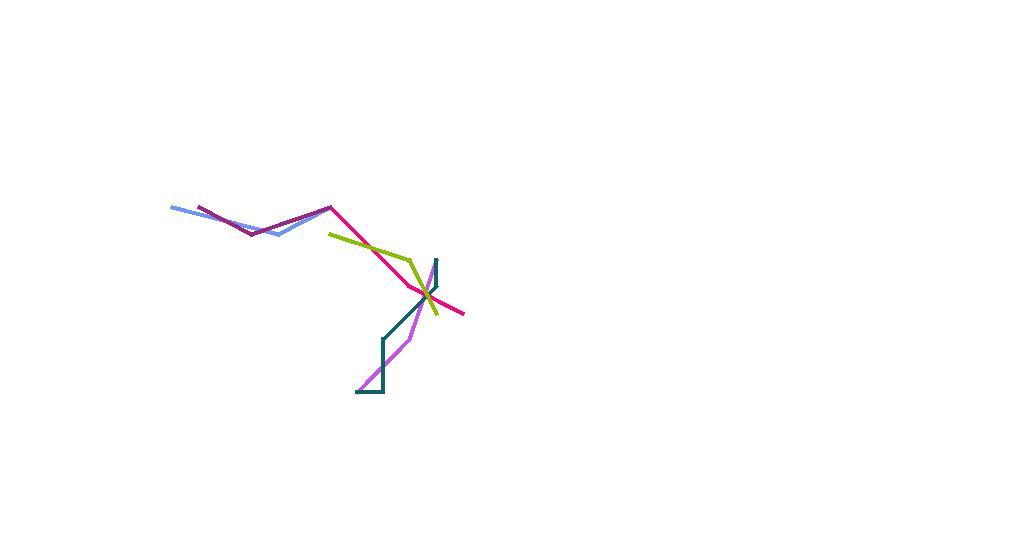
\includegraphics[width=0.85\linewidth]{1-6.png}}
% \end{figure*}
% 
% 
% \begin{figure*}[p]
% \fbox{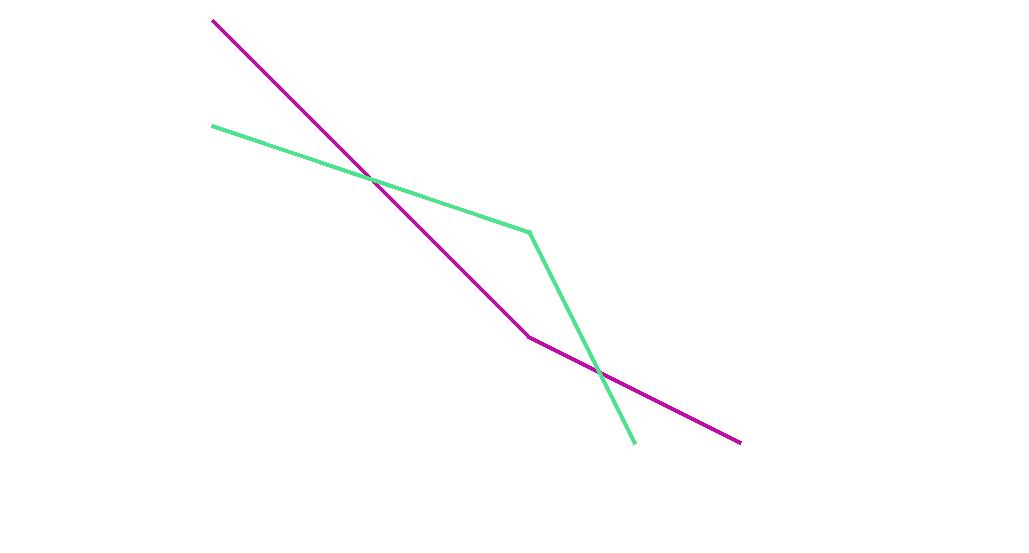
\includegraphics[width=0.65\linewidth]{3-4.png}}
% \end{figure*}
% 


% \section{User-interfaces}
% 
% 
% 
% 
% \framebox[4in][l]{\prompt \cmd{this is a command, short}}


\section{Test0.dat}



\vspace{-7\baselineskip}\footnotetext{You must download the program and the example data set, please see to page \pageref{download}.}
\vspace{7\baselineskip}




First of all, we must open the program (see page \pageref{openprogram}), read the data set and define the values of the parameters, to be used in this analysis. 

There are five parameters: \tui{c}ut value, 

three \tui{r}ules of decision,  and the value for \tui{m}inimal congruence.

For test0.dat we will use the following values:

\begin{center}
\begin{tabular}{ll}
\tui{c}ut & 0.25\\
\tui{r}ules & 0.75 0.5 1\\
\tui{m}inimal congruence & 0.8
\end{tabular}
\end{center}


\vspace{-7\baselineskip}\footnotetext{please remember:\\
to set each of these parameters you have to type the letters inside the square brackets [ ] and write the corresponding value followed by and enter}
\vspace{7\baselineskip}


\textbf{3. Search options}: Once the parameters have been defined, we will search the general patterns of distribution. 

As we might have similar initial MSTs, we need to find the similarity among the individual tracks to join a gro\tui{u}p of tracks according to the minimum value of \tui{m}inimal congruence fixed
 
In the case of test0.dat, we group from the track number 1 [first] to the track number 6 [last]. Thus, we find whether there are similar individual tracks that can be consider like the same track, and those tracks will be joint. 


Later, we need to redifined the values of the paramaters, in the case of test0.dat we will set:
\index{parameters:modify}


\begin{center}
\begin{tabular}{ll}
\tui{c}ut & 0.5\\
\tui{r}ules & 1.5 1 2\\
\tui{m}inimal congruence & 0.8
\end{tabular}
\end{center}



Then, Typing \tui{a}ll, we will find the congruent segments for each individual tracks in order to delimitate the generalized tracks or distributional patterns of species.

Finally, we need to eliminate those redundant generalized tracks, typing again \tui{u}, but joint from the track number 7  to the track 9, because first six tracks are individual tracks.

\textbf{4. write a kml file}

Now, we need to write our results (the generalized tracks) in a kml file. To do that, first we must type \tui{k} and \tui{+} to activate the output to the  kml file. The kml info must change from FALSE to TRUE. Then, we will use \tui{w} if we want to write the whole information of the analysis including: individual tracks, and generalized tracks, or we can type \tui{e} to write only the generalized tracks into the kml file.

\subsection{Command line interface}
\index{cli:command line interface}

For the command-line user interface we need to specified: the input file, output file, and parameters file.


For linux 64 bits:

\framebox[4.4in][l] {\prompt \cmd{ ./{\mt}-64 <input file> <output file> <parameters file>}}


%
%For linux 32 bits:
%
%\framebox[4.4in][l] {\prompt \cmd{ ./{\mt}-32 <input file> <output file> <parameters file>}}
%


For Windows 64 bits:

\framebox[4.5in][l] {\prompt \cmd{ {\mt}-64.exe <input file> <output file> <parameters file>}}


For Windows 64 bits:

\framebox[4.5in][l] {\prompt \cmd{ {\mt}-32.exe <input file> <output file> <parameters file>}}


\textbf{Output file:} it must have an extension .kml. 
\vspace{-7\baselineskip}\footnotetext{.kml file extension is mandatory with googleearth, otherwise googleearth will complain and will not open the file}
\vspace{7\baselineskip}


\textbf{parameters file:} This interface was designed for parameters/searching strategies defined previously. These search strategies have to be set in the parameters file. There are two main predefined strategies, \pname{croizat0}, and \pname{croizat1}.

\vspace{-7\baselineskip}\footnotetext{
CL typography: commands will be  \pname{croizat0}, to indicate that the instruction is named Croizat0 and you must type \pname{croizat0} in your parameter file, the command could be written using lower or upper case.}
\vspace{7\baselineskip}




The framework of \pname{croizat0} is: 
\begin{enumerate}
 \item Find similar individual tracks [=\tui{u}] from the first, to the last individual track
 \item Calculate the congruent segments among individual tracks (delimitate generalized tracks) [= \tui{a}]
 \item Find similar generalized tracks  [=\tui{u}] from the first, to the last generalized tracks
\end{enumerate}
Therefore, our analysis made with the TUI is a \pname{croizat0} analysis.


The framework of \pname{croizat1} is: 
\begin{enumerate}
 \item Calculate the congruent segments among individual tracks (delimitate generalized tracks) by \tui{a}
 \item Find similar generalized tracks by \tui{u} from the first, to the last generalized tracks
\end{enumerate}

Possible \textbf{parameters} values are: 
\index{parameters:values}
\vspace{-7\baselineskip}\footnotetext{
* cut value is a real <0 - 360> value expresed in degrees 

[0.0] = no cut - [360.0] = all points will be collapsed to one.


* rules  are real <0 - 360> values expresed in degrees


* minimal congruence is a real <0 - 1> value. 

[0.0] = no congruence - [1.0] = totally congruent.


please refer to our paper (cite) for further information}
\vspace{7\baselineskip}

\begin{center}
\begin{tabular}{lll}
\tui{c}ut & &\pname{set cut <real value 0-360>} \\
\tui{r}ules & lmax & \pname{set lmax <real value 0-360>}\\
 & lmin & \pname{set lmin  <real value 0-360>}\\
 & maxline & \pname{set maxline  <real value 0-360>}\\
\tui{m}inimal congruence & & \pname{set ci <real value 0-1>}
\end{tabular}
\end{center}



These values  are used to calculate the similarity among individual tracks in any analysis, joint or track.


Thus, the commands for the analysis of test0.dat, using par1-search1.txt are:
\index{running test0.dat}

For linux 64 bits:

\framebox[4.4in][l] {\prompt \cmd{ ./{\mt}-64 test0.dat test0.kml par1-search1.txt}}


For linux 32 bits:

\framebox[4.4in][l] {\prompt \cmd{ ./{\mt}-32 test0.dat test0.kml par1-search1.txt}}


For Windows 64 bits:

\framebox[4.5in][l] {\prompt \cmd{ {\mt}-64.exe test0.dat test0.kml par1-search1.txt}}


For Windows 64 bits:

\framebox[4.5in][l] {\prompt \cmd{ {\mt}-32.exe test0.dat test0.kml par1-search1.txt}}



\subsection{Results of test0.dat analysis}


\begin{figure}[!ht]
\begin{center}
 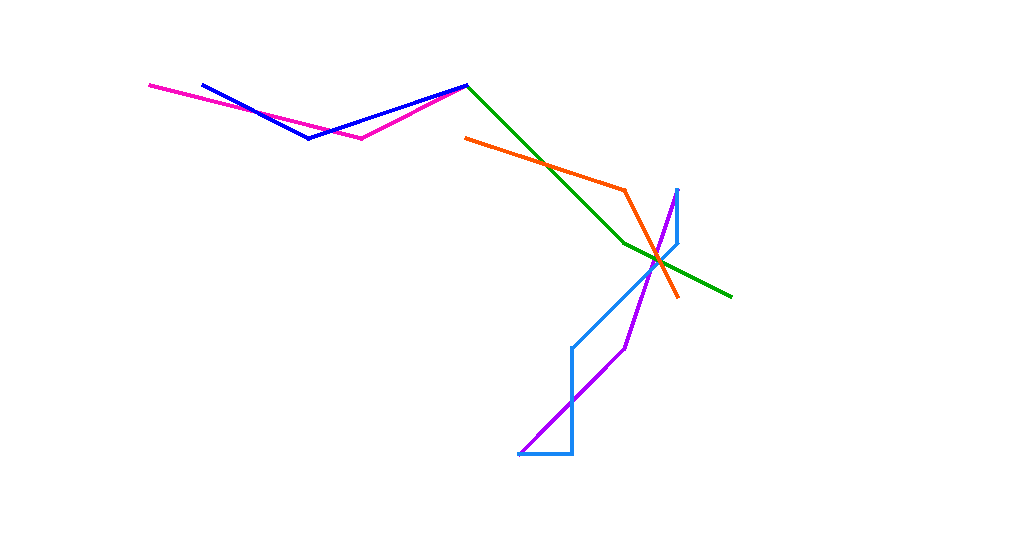
\includegraphics[scale=0.5]{./graphics/mst.png}
 % mst.png: 1029x553 pixel, 96dpi, 27.22x14.63 cm, bb=0 0 772 415
\end{center}
\caption{{\bf Individual tracks from test0.dat}}
\label{Figure1}
\end{figure}


\begin{figure}[!ht]
\begin{center}
 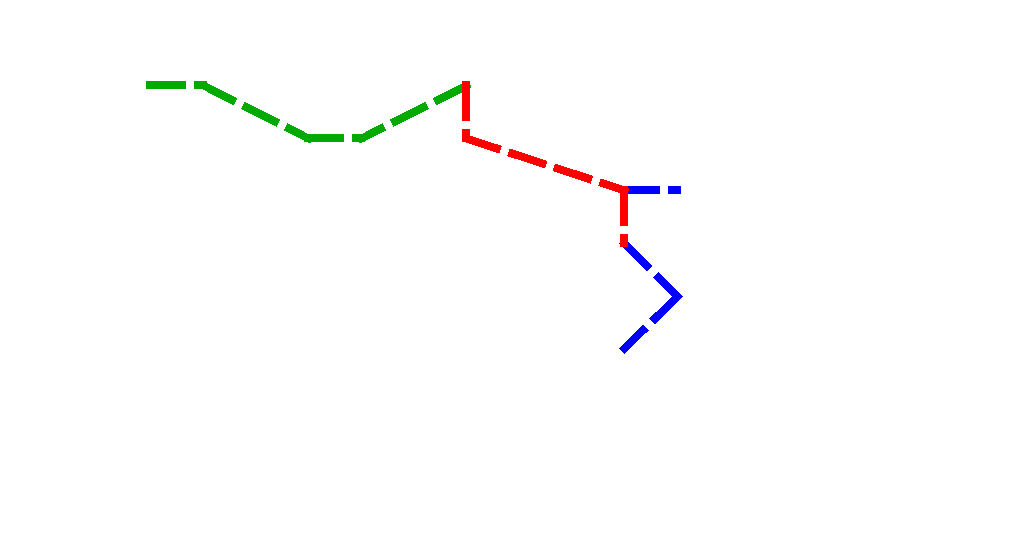
\includegraphics[scale=0.5]{./graphics/gtrack.png}
 % gtrack.png: 1029x553 pixel, 96dpi, 27.22x14.63 cm, bb=0 0 772 415
\end{center}
\caption{{\bf Generalized tracks from test0.dat}}
\label{Figure2}
\end{figure}

